\documentclass{standalone}
\usepackage{tikz}
\usetikzlibrary{patterns, positioning}

\begin{document}
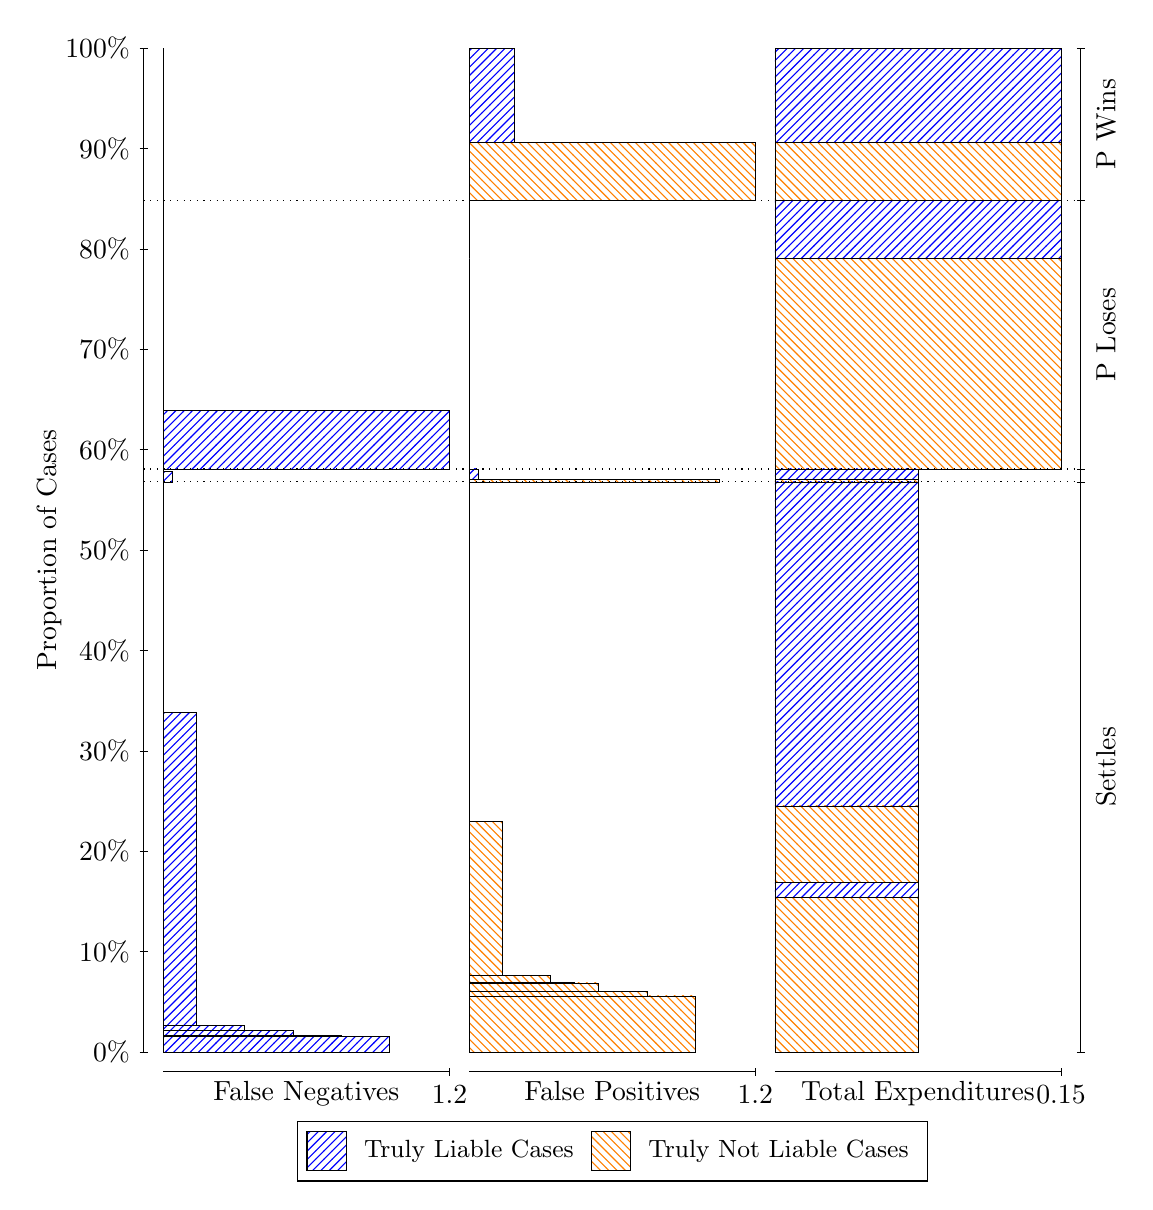
\begin{tikzpicture}
\draw[black, very thin] (1.5,1.75) -- (1.5,14.5);
\node[rotate=90, anchor=center] at (0.3, 8.125) {Proportion of Cases};
\draw[black, very thin] (1.45,1.75) -- (1.55,1.75);
\node[anchor=east] at (1.45, 1.75) {0\%};
\draw[black, very thin] (1.45,3.025) -- (1.55,3.025);
\node[anchor=east] at (1.45, 3.025) {10\%};
\draw[black, very thin] (1.45,4.3) -- (1.55,4.3);
\node[anchor=east] at (1.45, 4.3) {20\%};
\draw[black, very thin] (1.45,5.575) -- (1.55,5.575);
\node[anchor=east] at (1.45, 5.575) {30\%};
\draw[black, very thin] (1.45,6.85) -- (1.55,6.85);
\node[anchor=east] at (1.45, 6.85) {40\%};
\draw[black, very thin] (1.45,8.125) -- (1.55,8.125);
\node[anchor=east] at (1.45, 8.125) {50\%};
\draw[black, very thin] (1.45,9.4) -- (1.55,9.4);
\node[anchor=east] at (1.45, 9.4) {60\%};
\draw[black, very thin] (1.45,10.675) -- (1.55,10.675);
\node[anchor=east] at (1.45, 10.675) {70\%};
\draw[black, very thin] (1.45,11.95) -- (1.55,11.95);
\node[anchor=east] at (1.45, 11.95) {80\%};
\draw[black, very thin] (1.45,13.225) -- (1.55,13.225);
\node[anchor=east] at (1.45, 13.225) {90\%};
\draw[black, very thin] (1.45,14.5) -- (1.55,14.5);
\node[anchor=east] at (1.45, 14.5) {100\%};

\draw[black, very thin] (13.4,1.75) -- (13.4,14.5);
\draw[black, very thin] (13.35,1.75) -- (13.45,1.75);
\node[anchor=west] at (13.35, 1.75) {};
\draw[black, very thin] (13.35,8.9911) -- (13.45,8.9911);
\node[anchor=west] at (13.35, 8.9911) {};
\draw[black, very thin] (13.35,9.1538) -- (13.45,9.1538);
\node[anchor=west] at (13.35, 9.1538) {};
\draw[black, very thin] (13.35,12.569) -- (13.45,12.569);
\node[anchor=west] at (13.35, 12.569) {};
\draw[black, very thin] (13.35,14.5) -- (13.45,14.5);
\node[anchor=west] at (13.35, 14.5) {};

\draw[black, very thin, pattern color=blue, pattern=north east lines] (1.75,1.75) rectangle (4.6184,1.9433);
\draw[black, very thin, pattern color=blue, pattern=north east lines] (1.75,1.9433) rectangle (4.3125,1.9437);
\draw[black, very thin, pattern color=blue, pattern=north east lines] (1.75,1.9437) rectangle (4.0065,1.9633);
\draw[black, very thin, pattern color=blue, pattern=north east lines] (1.75,1.9633) rectangle (3.7005,1.9638);
\draw[black, very thin, pattern color=blue, pattern=north east lines] (1.75,1.9638) rectangle (3.3946,2.0196);
\draw[black, very thin, pattern color=blue, pattern=north east lines] (1.75,2.0196) rectangle (3.0886,2.0203);
\draw[black, very thin, pattern color=blue, pattern=north east lines] (1.75,2.0203) rectangle (2.7826,2.0855);
\draw[black, very thin, pattern color=blue, pattern=north east lines] (1.75,2.0855) rectangle (2.1707,6.0583);
\draw[black, very thin, pattern color=orange, pattern=north west lines] (1.75,6.0583) rectangle (1.75,8.9911);
\draw[black, very thin, pattern color=blue, pattern=north east lines] (1.75,8.9911) rectangle (1.8647,9.1197);
\draw[black, very thin, pattern color=orange, pattern=north west lines] (1.75,9.1197) rectangle (1.75,9.1538);
\draw[black, very thin, pattern color=blue, pattern=north east lines] (1.75,9.1538) rectangle (5.3833,9.8963);
\draw[black, very thin, pattern color=orange, pattern=north west lines] (1.75,9.8963) rectangle (1.75,12.569);
\draw[black, very thin, pattern color=orange, pattern=north west lines] (1.75,12.569) rectangle (1.75,13.305);
\draw[black, very thin, pattern color=blue, pattern=north east lines] (1.75,13.305) rectangle (1.75,14.5);
\draw[black, very thin, pattern color=orange, pattern=north west lines] (5.6333,1.75) rectangle (8.5018,2.4628);
\draw[black, very thin, pattern color=orange, pattern=north west lines] (5.6333,2.4628) rectangle (7.8898,2.5161);
\draw[black, very thin, pattern color=orange, pattern=north west lines] (5.6333,2.5161) rectangle (7.5839,2.5169);
\draw[black, very thin, pattern color=orange, pattern=north west lines] (5.6333,2.5169) rectangle (7.2779,2.6288);
\draw[black, very thin, pattern color=orange, pattern=north west lines] (5.6333,2.6288) rectangle (6.9719,2.6298);
\draw[black, very thin, pattern color=orange, pattern=north west lines] (5.6333,2.6298) rectangle (6.666,2.722);
\draw[black, very thin, pattern color=orange, pattern=north west lines] (5.6333,2.722) rectangle (6.36,2.7231);
\draw[black, very thin, pattern color=orange, pattern=north west lines] (5.6333,2.7231) rectangle (6.054,4.6828);
\draw[black, very thin, pattern color=blue, pattern=north east lines] (5.6333,4.6828) rectangle (5.6333,8.9911);
\draw[black, very thin, pattern color=orange, pattern=north west lines] (5.6333,8.9911) rectangle (8.8077,9.0252);
\draw[black, very thin, pattern color=blue, pattern=north east lines] (5.6333,9.0252) rectangle (5.7481,9.1538);
\draw[black, very thin, pattern color=orange, pattern=north west lines] (5.6333,9.1538) rectangle (5.6333,11.826);
\draw[black, very thin, pattern color=blue, pattern=north east lines] (5.6333,11.826) rectangle (5.6333,12.569);
\draw[black, very thin, pattern color=orange, pattern=north west lines] (5.6333,12.569) rectangle (9.2667,13.305);
\draw[black, very thin, pattern color=blue, pattern=north east lines] (5.6333,13.305) rectangle (6.207,14.5);
\draw[black, very thin, pattern color=orange, pattern=north west lines] (9.5167,1.75) rectangle (11.333,3.7108);
\draw[black, very thin, pattern color=blue, pattern=north east lines] (9.5167,3.7108) rectangle (11.333,3.9045);
\draw[black, very thin, pattern color=orange, pattern=north west lines] (9.5167,3.9045) rectangle (11.333,4.8766);
\draw[black, very thin, pattern color=blue, pattern=north east lines] (9.5167,4.8766) rectangle (11.333,8.9911);
\draw[black, very thin, pattern color=orange, pattern=north west lines] (9.5167,8.9911) rectangle (11.333,9.0252);
\draw[black, very thin, pattern color=blue, pattern=north east lines] (9.5167,9.0252) rectangle (11.333,9.1538);
\draw[black, very thin, pattern color=orange, pattern=north west lines] (9.5167,9.1538) rectangle (13.15,11.826);
\draw[black, very thin, pattern color=blue, pattern=north east lines] (9.5167,11.826) rectangle (13.15,12.569);
\draw[black, very thin, pattern color=orange, pattern=north west lines] (9.5167,12.569) rectangle (13.15,13.305);
\draw[black, very thin, pattern color=blue, pattern=north east lines] (9.5167,13.305) rectangle (13.15,14.5);
\draw[black, dotted] (1.5,8.9911) -- (13.4,8.9911);
\draw[black, dotted] (1.5,9.1538) -- (13.4,9.1538);
\draw[black, dotted] (1.5,12.569) -- (13.4,12.569);
\draw[black, very thin] (1.75,1.5) -- (5.3833,1.5);
\node[anchor=north] at (3.5667, 1.5) {False Negatives};
\draw[black, very thin] (5.3833,1.45) -- (5.3833,1.55);
\node[anchor=north] at (5.3833, 1.45) {1.2};

\draw[black, very thin] (5.6333,1.5) -- (9.2667,1.5);
\node[anchor=north] at (7.45, 1.5) {False Positives};
\draw[black, very thin] (9.2667,1.45) -- (9.2667,1.55);
\node[anchor=north] at (9.2667, 1.45) {1.2};

\draw[black, very thin] (9.5167,1.5) -- (13.15,1.5);
\node[anchor=north] at (11.333, 1.5) {Total Expenditures};
\draw[black, very thin] (13.15,1.45) -- (13.15,1.55);
\node[anchor=north] at (13.15, 1.45) {0.15};

\node[black, centered, rotate=90] at (13.72, 5.3706) {Settles};

\node[black, centered, rotate=90] at (13.72, 10.861) {P Loses};
\node[black, centered, rotate=90] at (13.72, 13.534) {P Wins};

\draw (7.449999999999999,1.5) node[draw=none] (baseCoordinate) {};
\begin{scope}[align=center]
        \matrix[scale=0.5, draw=black, below=0.5cm of baseCoordinate, nodes={draw}, column sep=0.1cm]{
            \node[rectangle, draw, minimum width=0.5cm, minimum height=0.5cm, pattern=north east lines, pattern color=blue] {}; &
            \node[draw=none, font=\small] (B) {Truly Liable Cases}; &
            \node[rectangle, draw, minimum width=0.5cm, minimum height=0.5cm, pattern=north west lines, pattern color=orange] {}; &
            \node[draw=none, font=\small] (B) {Truly Not Liable Cases}; \\
            };
\end{scope}

\end{tikzpicture}
\end{document}